\documentclass[a4paper,10pt]{article}

\usepackage[margin=20mm]{geometry}
\usepackage{graphicx}
\usepackage{url}
\usepackage{setspace}

\title{Time Block Tracker：時間ブロックとポモドーロによる学習時間記録ツール}
\author{LIU SIQI \\ 学籍番号：268e151e}
\date{7/13}

\begin{document}

\maketitle

\section{目的}

本ソフトウェアは，日々の学習・作業時間を記録し，自分の時間の使い方を振り返るための軽量なコマンドラインツールである。
一般的なToDo管理では「何をするか」を管理することが多いが，実際にどれだけの時間を使ったかは把握しにくい。
そこで本ソフトウェアでは，一日を大きな時間ブロックに分けて記録する方法と，ポモドーロ形式の集中作業を記録する方法を組み合わせた。

GitHubリポジトリは以下である。

\begin{center}
\url{https://github.com/268e151e-hub/time-block-tracker}
\end{center}

\section{実装上の工夫}

本ソフトウェアはPythonで実装し，データの保存にはCSVを用いた。
CSVを用いることで，ユーザーは記録されたデータを表計算ソフトでも確認できる。
また，集計にはpandas，グラフの作成にはMatplotlibを用いた。

主な機能は次の三つである。
第一に，\texttt{timeblock add-block} によって，morningやafternoonなどの定義済み時間ブロックを記録できる。
第二に，\texttt{timeblock add-pomodoro} によって，25分などのポモドーロ形式の集中時間を記録できる。
第三に，\texttt{timeblock summary} と \texttt{timeblock plot} によって，記録の集計とPDF形式のグラフ作成ができる。

保守性を高めるため，記録の追加，集計，グラフ作成をそれぞれ \texttt{core.py}，\texttt{plot.py}，\texttt{cli.py} に分けて実装した。
また，pytestによる単体テストを作成し，GitHub ActionsによるCIを設定した。
これにより，pushするたびに自動でテストが実行される。

\section{検証}

本ソフトウェアが目的を達成できたかを確認するため，実際に学習時間の記録を行い，カテゴリ別の集計グラフを作成した。
例として，日本語学習の時間ブロックと，プログラミング学習のポモドーロ記録を入力した。
その結果，カテゴリごとの合計時間が自動的に計算され，図\ref{fig:category}のようにPDF形式で可視化された。

\begin{figure}[h]
    \centering
    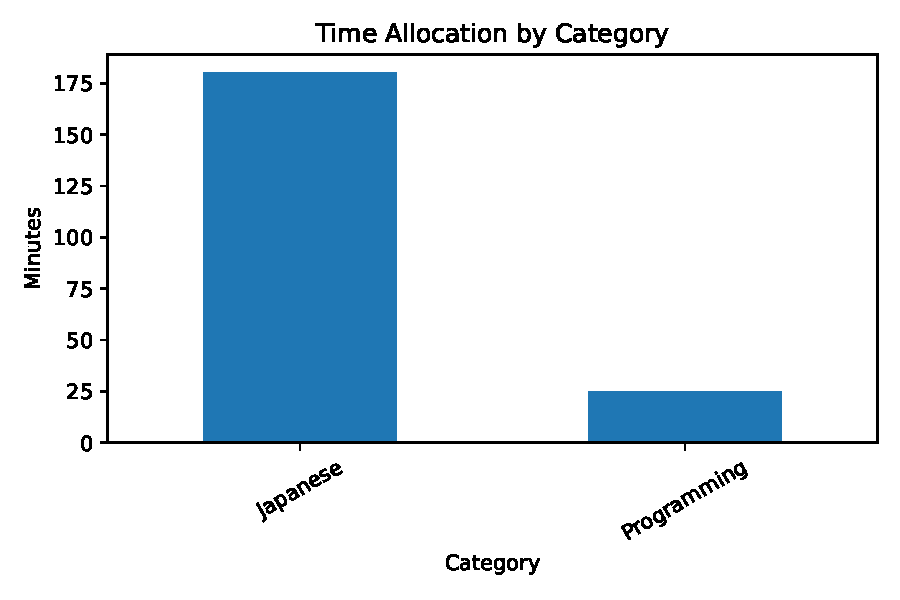
\includegraphics[width=0.75\linewidth]{../reports/category_summary.pdf}
    \caption{カテゴリ別の記録時間}
    \label{fig:category}
\end{figure}

手作業で学習時間を集計する場合，記録を見直し，カテゴリごとに時間を足し合わせる必要がある。
一方，本ソフトウェアでは，記録の追加後に \texttt{timeblock summary} または \texttt{timeblock plot} を実行するだけで集計と可視化が完了する。
したがって，本ソフトウェアは，日々の時間使用を簡単に記録し，学習時間を振り返るという目的を達成している。

\section{AIの使用について}

本課題では，ChatGPTを使用した。
主に，ソフトウェアのテーマ設計，プロジェクト構成の検討，Pythonコードの作成補助，pytestのテスト方針，READMEの構成，LaTeXレポートの文章整理に利用した。
ただし，生成されたコードはそのまま提出するのではなく，実際にCodespaces上で実行し，pytestとGitHub Actionsで動作確認を行った。
また，エラーが発生した場合には，エラーメッセージを確認しながら修正した。

\end{document}